\documentclass[11pt]{article}
\usepackage{matt}
\begin{document}

\section*{Update for the Week of \today}

\begin{figure}[h]
  \centering
  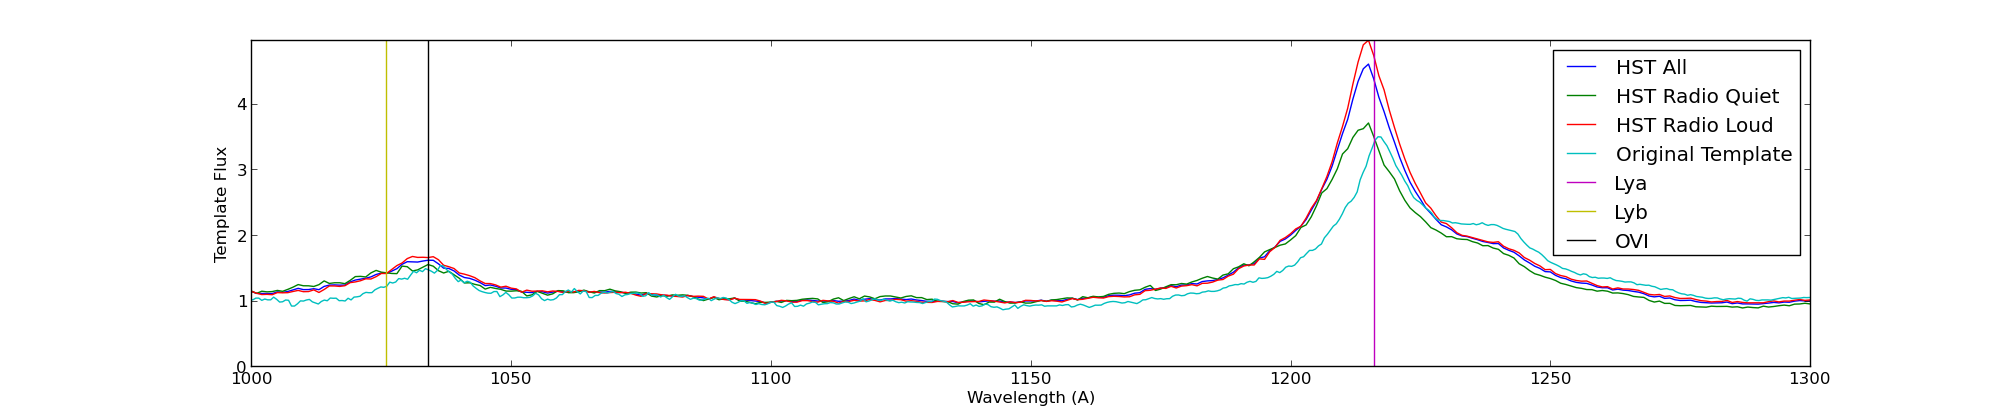
\includegraphics[width=18cm]{CompareTemplates.png}
  \caption{todo}
  \label{fig:todo}
\end{figure}


\begin{figure}[h]
  \centering
  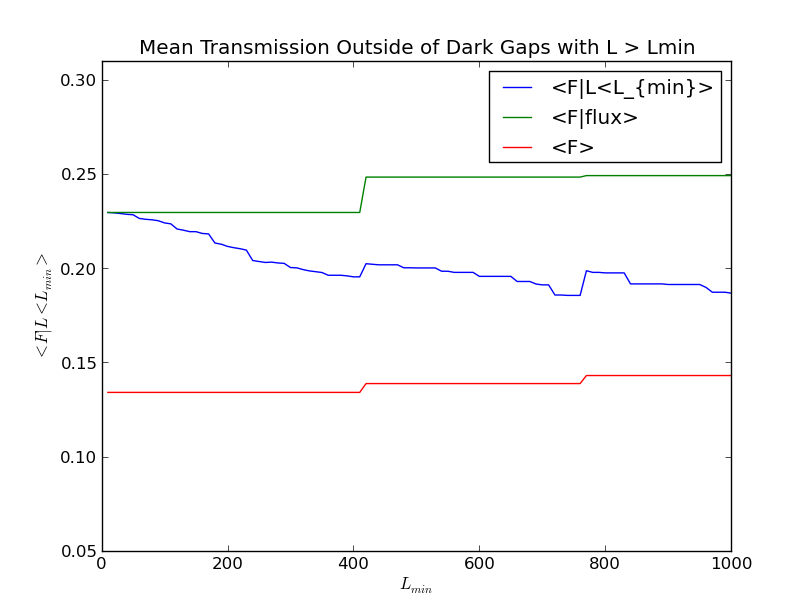
\includegraphics[width=8cm]{flux_ExcludeLs.png}
  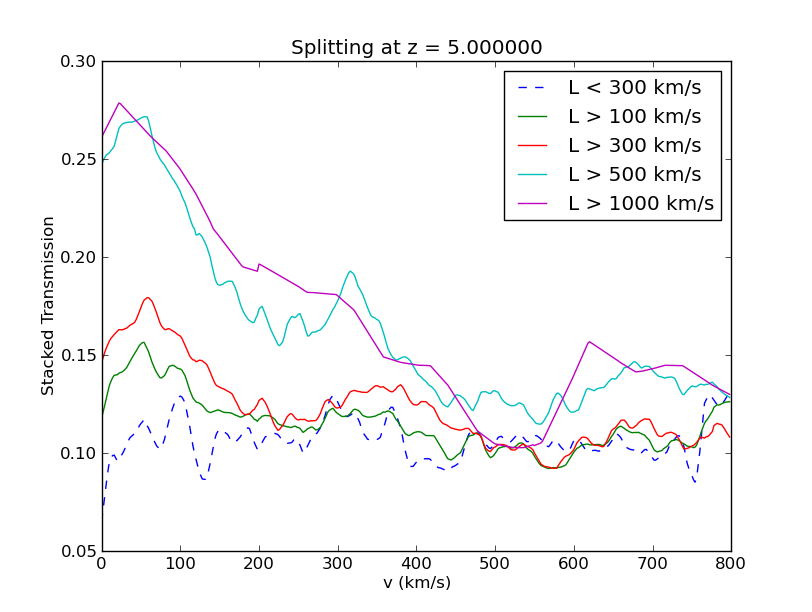
\includegraphics[width=8cm]{Stack_Zgreaterthan5.png}
  \caption{The left-hand figure shows several measures of mean transmission for the spectra used in our stack. The red line shows the overall mean transmission \textit{for spectra that contain at least one dark gap with $L > L_{\text{min}}$}. The blue curve shows the mean transmission for spectra with at least one dark gap with $L > L_{\text{min}}$, but \textit{masking dark gaps with $L > L_{\text{min}}$}. The green curve shows the mean transmission in regions \textit{with} transmission for spectra that have at least one dark gap with $L > L_{\text{min}}$. We would na\"ively expect the stacked transmission to begin at the level of the green line in the left-hand figure and level off to that of the red line, which is seen for the $L_{\text{min}} \gtrsim 500\kms$ case, but not for the others.}
  \label{fig:todo}
\end{figure}


\end{document}